\documentclass[conference]{IEEEtran}
\IEEEoverridecommandlockouts
% ----------------------------------------------------------------------
% Packages
% ----------------------------------------------------------------------
\usepackage{cite}
\usepackage{amsmath,amssymb,amsfonts}
\usepackage{graphicx}
\usepackage{textcomp}
\usepackage{xcolor}
\usepackage{booktabs}
\usepackage{url}
\usepackage{tikz}
\usetikzlibrary{arrows.meta, positioning}
\usepackage{placeins}
\graphicspath{{figures/}}

\def\BibTeX{{\rm B\kern-.05em{\sc i\kern-.025em b}\kern-.08em
    T\kern-.1667em\lower.7ex\hbox{E}\kern-.125emX}}

\begin{document}

% ----------------------------------------------------------------------
% Title and authors
% ----------------------------------------------------------------------
\title{Integrating Adaptive Neuro-Fuzzy Inference Systems and Large Language Models for Arabic Dialect Processing}

\author{
\IEEEauthorblockN{1\textsuperscript{st} Ibrahim Youssef El-Noshokaty}
\IEEEauthorblockA{\parbox{3.7cm}{\centering\small
\textit{Acoustics\&Artificial Intelligence}\\
\textit{Enosh Science Research Center}\\
Cairo, Egypt\\
ibrahim@enoshscience.com\\
\scriptsize https://orcid.org/0000-0002-3544-9129}}
\and
\IEEEauthorblockN{2\textsuperscript{nd} Shaimaa EL-Ragae}
\IEEEauthorblockA{\parbox{3.7cm}{\centering\small
\textit{Assistant Professor and Quality Assurance Officer}\\
\textit{Enosh Science Research Center}\\
Cairo, Egypt\\
shaima.rageay@enoshscience.com\\
\scriptsize https://orcid.org/009-0006-2184-5477}}
\and
\IEEEauthorblockN{3\textsuperscript{rd} Rahma Mohamed Mohamed}
\IEEEauthorblockA{\parbox{3.7cm}{\centering\small
\textit{Acoustics\&Artificial Intelligence}\\
\textit{Enosh Science Research Center}\\
Cairo, Egypt\\
Rahma.mohamed@enoshscience.com\\
\scriptsize https://orcid.org/0009-0008-2878-160X}}
}

\maketitle

% ----------------------------------------------------------------------
% Abstract and keywords
% ----------------------------------------------------------------------
\begin{abstract}
Arabic poses ongoing difficulties for Natural Language Processing (NLP) because of its intricate morphology, complex writing system, and wide range of dialects. This research explores a hybrid framework that combines Adaptive Neuro-Fuzzy Inference Systems (ANFIS) with Large Language Models (LLMs) to process Arabic dialects. Utilizing a gold-standard dataset crafted by experts, which includes 999 dialogue scenarios in three parallel dialects---Levantine (LEV), Egyptian (EGY), and Gulf (GUL)---we examine 2,997 pairs of utterances and responses. Sentence embeddings are generated using the sentence-transformers/paraphrase-multilingual-MiniLM-L12-v2 model and are then reduced to 50 dimensions through Principal Component Analysis (PCA), maintaining 75.38\% and 75.19\% of the variance for utterances and responses, respectively. Visualizations using t-Distributed Stochastic Neighbor Embedding (t-SNE) show a distinct and compact GUL cluster, while LEV and EGY display significant overlap, consistent with previous studies on the similarity of Arabic dialects. In the PCA space, centroid analysis reveals that the distances between LEV and GUL are the greatest (3.1997 for utterances, 2.6905 for responses), while those between EGY and GUL are the smallest (2.8160, 2.4971), and the distances between LEV and EGY fall in between (2.9083, 2.5673). This indicates a distinct GUL region and a somewhat indistinct boundary between LEV and EGY. Utilizing this framework, we establish a continuous dialect axis and introduce an ANFIS layer that translates embeddings into fuzzy membership degrees $\mu_d$, with the sum $\sum_d \mu_d \approx 1$, to manage an LLM decoder. We train and evaluate this layer directly: a zero-order Sugeno ANFIS with an anisotropic Gaussian premise and a learned defuzzification (consequent) layer is fit on an 80/20 stratified train/test split (with all projections fit on training data only) over embeddings from a dialect-specialized encoder (MARBERT), achieving 85.33\% held-out three-way dialect-classification accuracy---well above chance, above a $k$-nearest-neighbor baseline (79.00\%) on the same embeddings, and substantially above an isotropic-premise variant on the identical features (65.83\%), with balanced recall across all three dialects (83--89\%). Beyond this classification result, we instantiate the proposed ANFIS--LLM architecture as a working closed loop: the trained fuzzy membership degrees $\mu_d$ are converted into a dialect-aware steering prompt that conditions an LLM decoder, which we demonstrate on held-out utterances---producing dialect-appropriate Arabic responses---and in ENOSH, a live interactive demo, confirming that these membership degrees carry genuine, actionable dialectal signal rather than remaining a purely conceptual construct. Because the utterances and responses are parallel, topic-matched translations of the same 999 scenarios across dialects, these findings characterize the structure of dialectal variation captured by multilingual Transformer embeddings within this controlled, matched corpus; we do not claim generalization to naturally occurring, topic-unmatched Arabic text, which is left to future work with an external corpus. Within this scope, the findings illustrate gradual transition zones between dialects that are more accurately represented by neuro-fuzzy membership than by rigid labels. This approach facilitates the development of context-aware, dialect-sensitive dialogue systems based on authentic conversational benchmarks.
\end{abstract}

\begin{IEEEkeywords}
Arabic dialects, large language models, neuro-fuzzy inference, sentence embeddings, dialect identification, dialogue systems
\end{IEEEkeywords}

% ----------------------------------------------------------------------
\section{Introduction}
The Arabic language, with its rich morphology, complex orthography, and extensive dialectal diversity, poses a distinctive set of challenges for Natural Language Processing (NLP) systems \cite{habash2012}, \cite{elhaj2021}. Beyond Modern Standard Arabic (MSA), everyday communication relies heavily on regional dialects---Egyptian, Levantine, Gulf, Maghrebi, and others---each with distinct phonological, lexical, and syntactic patterns \cite{altwairesh2018} that diverge substantially from MSA and from one another, with less standardized written forms. Dialect boundaries are often ``fuzzy'' rather than discrete, especially amid code-switching and informal spelling, and even powerful Large Language Models (LLMs) can generate technically correct but dialectally inappropriate responses in such settings \cite{reimers2019}, degrading user experience and losing socio-linguistic nuance.

Adaptive Neuro-Fuzzy Inference Systems (ANFIS) offer a natural remedy: a hybrid framework combining the data-driven learning of neural networks with the interpretability and graded-membership strengths of fuzzy inference \cite{jang1993}, able to represent gradual transitions between dialects rather than forcing hard, categorical decisions. Layering ANFIS on top of LLM-derived embeddings lets a system infer graded dialect memberships and use them to adapt style and response generation to a user's inferred dialectal profile, rather than treating dialect identification as a single hard label.

This paper accordingly (a) characterizes the dialectal structure observable in embedding spaces derived from parallel dialogue data, (b) implements and empirically evaluates, on a held-out test set, an ANFIS layer that converts these embeddings into fuzzy dialect-membership degrees, and (c) instantiates this layer in a working closed-loop pipeline that steers an LLM decoder toward dialect-appropriate generation.

% ----------------------------------------------------------------------
\section{Methodology}
This work implements a reproducible pipeline for analyzing dialectal variation across three major Arabic dialects---Levantine (LEV), Egyptian (EGY), and Gulf (GUL)---which diverge from Modern Standard Arabic and from one another in lexicon, morphology, and syntax \cite{habash2012}, \cite{elhaj2021}. Sentence-level representations are obtained with a Sentence Transformer \cite{reimers2019}, examined via Principal Component Analysis (PCA) and t-SNE \cite{jolliffe2002}, \cite{vandermaaten2008}, and used to train an Adaptive Neuro-Fuzzy Inference System (ANFIS) layer \cite{jang1993} that estimates graded dialect membership. Figure~\ref{fig:architecture} summarizes the resulting layered ANFIS--LLM architecture: embeddings, dimensionality reduction, fuzzy membership estimation, and dialect-adapted generation interacting within a unified pipeline.

The original dataset (\texttt{ARABIC\_DIALECTS\_\allowbreak ANFIS\_GOLD.xlsx}) was provided in a wide format, with separate columns for utterances and responses for each dialect (LEV, EGY, GUL). For analytical consistency, the data were converted into a long format with explicit columns: \texttt{dialect\_code}, \texttt{dialect\_name}, \texttt{utterance}, and \texttt{response}. To support later neuro-fuzzy modeling and numeric analysis, a continuous dialect encoding was introduced, defining a one-dimensional ``dialect axis'' on which each dialect occupies a distinct position between 0 and 1. This axis is defined by the mapping:

\begin{equation}
d_{LEV} = 0.0, \quad d_{EGY} = 0.5, \quad d_{GUL} = 1.0
\label{eq:axis}
\end{equation}

This mapping is a convenient notational device for graded membership, not a claim about the true geometry of dialect similarity. Fixed positions inevitably impose an ordering and equal spacing (LEV--EGY, EGY--GUL each 0.5; LEV--GUL 1.0) that our own centroid distances do not support: measured pairwise distances (Table~\ref{tab:centroids}) are of comparable magnitude across all three pairs rather than following this 2:1:1 ratio. We flag this honestly, following a reviewer's comment, and emphasize that the axis plays no role in any analysis that follows---centroid distances, t-SNE, and the ANFIS premise and classifier (Section~III onward) are all computed directly from the full 50-dimensional PCA embeddings, never through this one-dimensional projection.

For each utterance or response $s_i$, we obtain a 384-dimensional embedding $x_i = f_\theta(s_i) \in \mathbb{R}^{384}$ using sentence-transformers/paraphrase-multilingual-MiniLM-L12-v2 \cite{reimers2019}, with batch encoding for efficiency and consistency. Given the embedding matrix $X \in \mathbb{R}^{N \times 384}$ and its mean $\mu = \frac{1}{N}\sum_i x_i$, PCA computes an orthogonal projection matrix $W \in \mathbb{R}^{384 \times 50}$ from the top 50 principal components \cite{jolliffe2002}, giving

\begin{equation}
z_i = W^\top (x_i - \mu), \quad z_i \in \mathbb{R}^{50}.
\label{eq:pca}
\end{equation}

PCA preserved approximately 75.38\% of the variance for utterance embeddings and 75.19\% for response embeddings. For visualization, t-SNE \cite{vandermaaten2008} then maps these 50-dimensional outputs to two dimensions by minimizing the Kullback--Leibler divergence between pairwise-similarity distributions in the high- and low-dimensional spaces, highlighting dialect clusters and overlaps. To quantify separation, we compute each dialect's centroid $c_k = \frac{1}{N_k}\sum_{i \in D_k} z_i$ in this 50-dimensional space.

The Euclidean distance $d(c_k,c_\ell) = \lVert c_k - c_\ell \rVert_2$ between two dialects' centroids indicates their separability: larger distances mean less overlap. In the present study, the LEV--GUL pair consistently showed the largest centroid distances, whereas the EGY--GUL pair exhibited the smallest, aligning with prior observations on Arabic dialect variation \cite{altwairesh2018}, \cite{elhaj2021}.

To test whether this centroid separation could plausibly arise from chance alone, we ran a permutation test: we randomly shuffled the dialect labels 1,000 times and recomputed the average pairwise centroid distance under each shuffle. The observed average pairwise centroid distance under the true labels (0.389) substantially exceeds the distribution obtained under random shuffling (mean 0.117, std 0.011, maximum 0.157 across all 1,000 permutations), yielding $p = 0.001$. This indicates that the separation between dialect centroids is unlikely to be an artifact of chance, providing statistical support for the descriptive centroid analysis beyond the raw distance values alone.

% --- Figure 1: architecture diagram (recreated in TikZ) ---
\begin{figure}[t]
\centering
\resizebox{\columnwidth}{!}{%
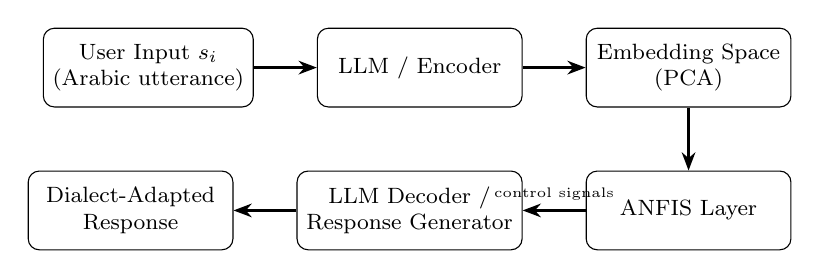
\begin{tikzpicture}[
  node distance = 8mm and 8mm,
  box/.style = {draw, rounded corners, align=center, minimum height=1cm, minimum width=2.6cm, font=\footnotesize},
  arrow/.style = {-{Stealth}, thick}
]
  \node[box] (input) {User Input $s_i$\\(Arabic utterance)};
  \node[box, right=of input] (llm) {LLM / Encoder};
  \node[box, right=of llm] (pca) {Embedding Space\\(PCA)};
  \node[box, below=of pca] (anfis) {ANFIS Layer};
  \node[box, left=of anfis] (decoder) {LLM Decoder /\\Response Generator};
  \node[box, left=of decoder] (output) {Dialect-Adapted\\Response};

  \draw[arrow] (input) -- (llm);
  \draw[arrow] (llm) -- (pca);
  \draw[arrow] (pca) -- (anfis);
  \draw[arrow] (anfis) -- node[above, font=\tiny]{control signals} (decoder);
  \draw[arrow] (decoder) -- (output);
\end{tikzpicture}}
\caption{Layered architecture of the proposed ANFIS--LLM hybrid system for Arabic multi-dialect dialogue processing.}
\label{fig:architecture}
\end{figure}

An input utterance $s_i$ in Arabic is first mapped by the encoder/LLM to a high-dimensional sentence embedding $x_i = f_\theta(s_i) \in \mathbb{R}^{384}$. Principal Component Analysis (PCA) then projects this representation into a lower-dimensional embedding space $z_i = W^\top(x_i - \mu) \in \mathbb{R}^{50}$. On top of this shared embedding space, the ANFIS layer estimates fuzzy dialect membership degrees $\mu_{LEV}(z_i)$, $\mu_{EGY}(z_i)$, and $\mu_{GUL}(z_i)$ in the range $[0,1]$, with $\mu_{LEV} + \mu_{EGY} + \mu_{GUL} \approx 1$. These neuro-fuzzy control signals are then used by the LLM decoder $\hat{y}_i = g(z_i, \mu_{dialect})$ to generate a dialect-adapted response $y_i$ that is semantically coherent and stylistically aligned with the inferred dialectal profile.

\subsection{Training and Evaluation of the ANFIS Layer}
To directly evaluate the fuzzy membership layer summarized in Fig.~\ref{fig:architecture}, we implemented and trained a zero-order Sugeno-type ANFIS classifier. The 2,997 utterance--response pairs were partitioned into training (80\%) and held-out test (20\%) sets by stratified sampling (seed 42); every projection and premise/consequent parameter below was fit exclusively on the training partition and applied to the held-out test partition, so no test information leaked into fitting.

For this classification sub-task, embeddings were generated with UBC-NLP/MARBERT \cite{abdulmageed2021}, a BERT-family model pretrained on dialectal Arabic tweets, rather than the general-purpose paraphrase-alignment model used for the exploratory analysis in Sections~III-A--III-B. This is a deliberate choice: the exploratory analysis benefits from a model trained to align semantically equivalent sentences, while classification benefits from an encoder explicitly trained to distinguish dialectal register; the two sub-components are free to use the representation best suited to their objective, and Sections~III-A--III-B are unaffected. As before (Eq.~\ref{eq:pca}), a 50-dimensional PCA projection was fit on the training partition only---retaining 73.88\% of variance in the MARBERT space.

For each dialect $d \in \{LEV, EGY, GUL\}$, we estimate an \emph{anisotropic} Gaussian premise membership function: rather than a single per-class variance scalar, each of the $D=50$ PCA dimensions $j$ receives its own class-conditional variance $\sigma_{d,j}^2$, estimated from the training embeddings assigned to dialect $d$ and floored at 5\% of the pooled (all-class) per-dimension variance $\bar\sigma_j^2$ to guard against numerically unstable estimates in dimensions with limited within-class spread:

\begin{equation}
\sigma_{d,j}^2 = \max\!\left(\operatorname{Var}_{i \in D_d}(z_{i,j}),\ 0.05\,\bar\sigma_j^2\right)
\label{eq:variance}
\end{equation}

Given a query embedding $z$, the log firing strength of rule $d$ under this anisotropic premise is

\begin{equation}
\log w_d(z) = -\frac{1}{2}\sum_{j=1}^{D} \log \sigma_{d,j}^2 - \sum_{j=1}^{D} \frac{(z_j - c_{d,j})^2}{2\sigma_{d,j}^2}
\label{eq:firing}
\end{equation}

and the fuzzy membership degree $\mu_d(z)$ is obtained by normalizing firing strengths across the three rules, $\mu_d(z) = w_d(z) / \sum_{k} w_k(z)$, so that $\sum_d \mu_d(z) = 1$. Unlike the isotropic premise of our initial submission, which treats all 50 PCA dimensions as equally informative, this anisotropic form lets strongly class-discriminative dimensions dominate the decision---an architectural change whose empirical effect is quantified in Section~III-C.

Finally, to complete the canonical five-layer Sugeno ANFIS pipeline rather than deciding directly from normalized membership degrees, we add an explicit \emph{defuzzification} (consequent) layer: a $3\times3$ matrix $R$ fit by ordinary least squares against one-hot training labels,
\begin{equation}
R = \operatorname*{arg\,min}_{R} \; \lVert Y_{\text{train}} - M_{\text{train}} R \rVert_F^2,
\label{eq:defuzz}
\end{equation}
where $M_{\text{train}}$ stacks training membership vectors $\mu(z_i)$ and $Y_{\text{train}}$ their one-hot labels. The defuzzified class scores for a query $z$ are $\mu(z)^\top R$, with the predicted dialect taken as $\arg\max$ over these scores rather than over $\mu(z)$ directly. As a baseline, we also evaluated a $k$-nearest-neighbor ($k$=5) classifier on the same embeddings and split.

% ----------------------------------------------------------------------
\section{Results and Discussion}
We distinguish two evaluation regimes throughout this section. Sections~III-A and III-B report a descriptive, unsupervised analysis (centroid distances and t-SNE) over the full corpus with no train/test split---appropriate for exploratory characterization but not predictive validation. Section~III-C then reports a separate, properly held-out supervised evaluation of the trained ANFIS classifier, with every parameter fit exclusively on a training partition and accuracy measured strictly on unseen test data (Section~II-A); this held-out evaluation, not the exploratory analysis, is what we offer as quantitative evidence of dialect separability.

\subsection{Quantitative Assessment: Inter-Dialect Centroid Distances}

\begin{table}[t]
\centering
\caption{Euclidean distances between PCA-reduced dialect centroids}
\label{tab:centroids}
\begin{tabular}{lcc}
\toprule
Dialect Pair & Utterance Centroid Dist. & Response Centroid Dist. \\
\midrule
LEV--EGY & 2.9083 & 2.5673 \\
LEV--GUL & 3.1997 & 2.6905 \\
EGY--GUL & 2.8160 & 2.4971 \\
\bottomrule
\end{tabular}
\end{table}

The LEV--GUL pair exhibited the largest centroid distances for both utterances (3.1997) and responses (2.6905), indicating that Levantine and Gulf Arabic are the most distinct within this embedding space, while EGY--GUL showed the smallest (2.8160, 2.4971), suggesting a comparatively closer relationship \cite{habash2012}, \cite{elhaj2021}.

\subsection{Qualitative Analysis: Visual Separation via t-SNE}
t-SNE visualizations were used to provide qualitative insight into how utterances and responses cluster by dialect in a two-dimensional space \cite{vandermaaten2008}. Fig.~\ref{fig:tsne_all} shows the distribution of all three dialects for both utterance and response embeddings.

\begin{figure}[t]
\centering
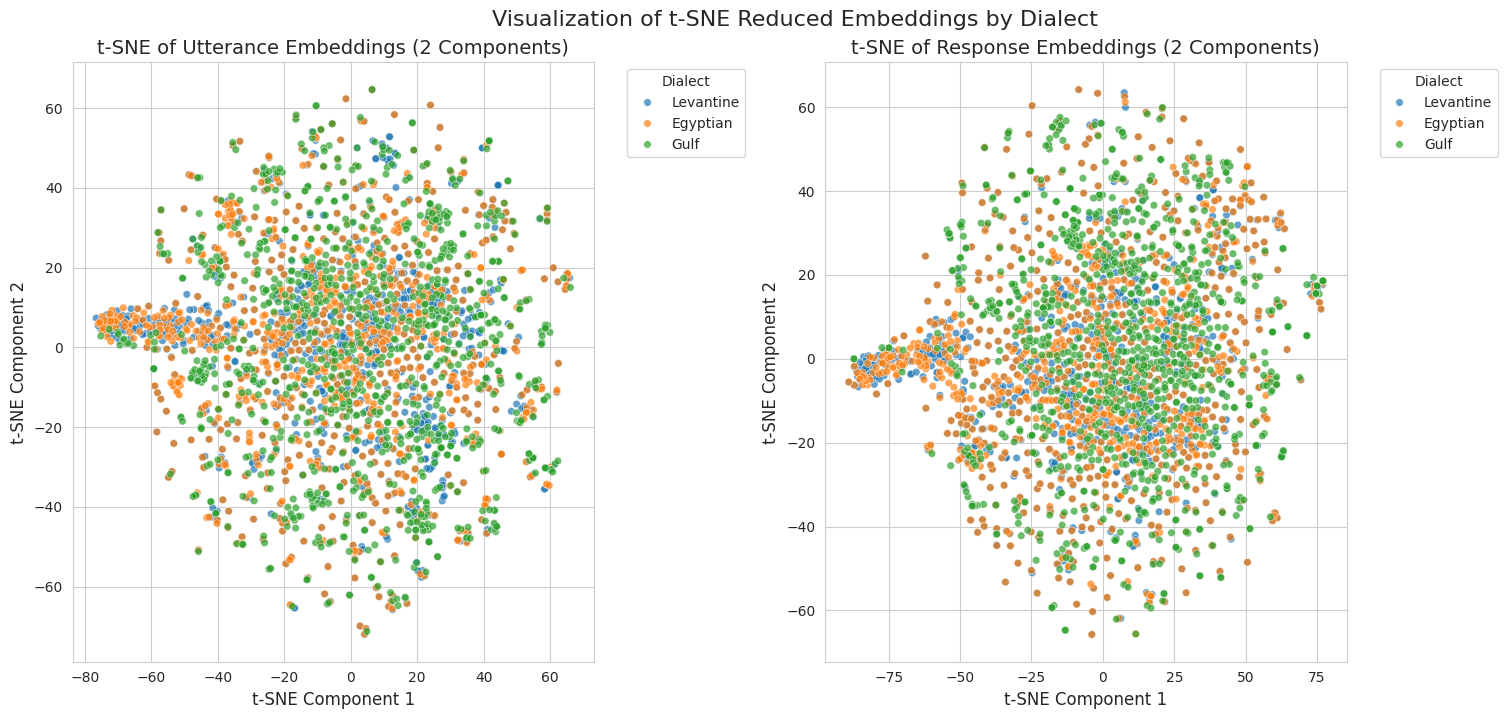
\includegraphics[width=\columnwidth]{figure2_tsne_all_dialects.png}
\caption{t-SNE visualization of utterance and response embeddings for Levantine, Egyptian, and Gulf dialects.}
\label{fig:tsne_all}
\end{figure}

In both utterance and response plots, Gulf Arabic (GUL) forms a comparatively more compact grouping with reduced overlap relative to LEV and EGY---which themselves show substantial overlap, particularly in utterance embeddings---broadly consistent with the centroid-distance results. We are careful not to over-interpret this visual pattern, however: t-SNE does not reliably preserve global distances or density, and closer inspection shows that some mixing among all three dialects persists even where GUL appears comparatively separated. We therefore treat these t-SNE plots as illustrative of the qualitative structure of the embedding space rather than as quantitative evidence of separability; the controlled classification experiment in Section~III-C, with held-out accuracy, a full confusion matrix, and a $k$-NN baseline, is what we offer as actual quantitative evidence of separability. Consistent with this caution, the silhouette score for the three dialect labels in this 50-dimensional PCA space is $-0.0189$---essentially zero, indicating that individual utterances are not cleanly separated point-by-point, even though their class centroids are significantly further apart than chance would predict (Section~III-A). We read these two statistics together: the dialects are not cleanly separable point-by-point in this unsupervised, whole-corpus space, which is precisely the kind of overlap that motivates a graded, fuzzy-membership treatment rather than a hard categorical one, while the supervised ANFIS classifier in Section~III-C, exploiting per-dimension structure a single global silhouette statistic cannot, still achieves well-above-chance held-out accuracy.

\subsection{ANFIS Dialect-Membership Evaluation}

\begin{figure*}[tb]
\centering
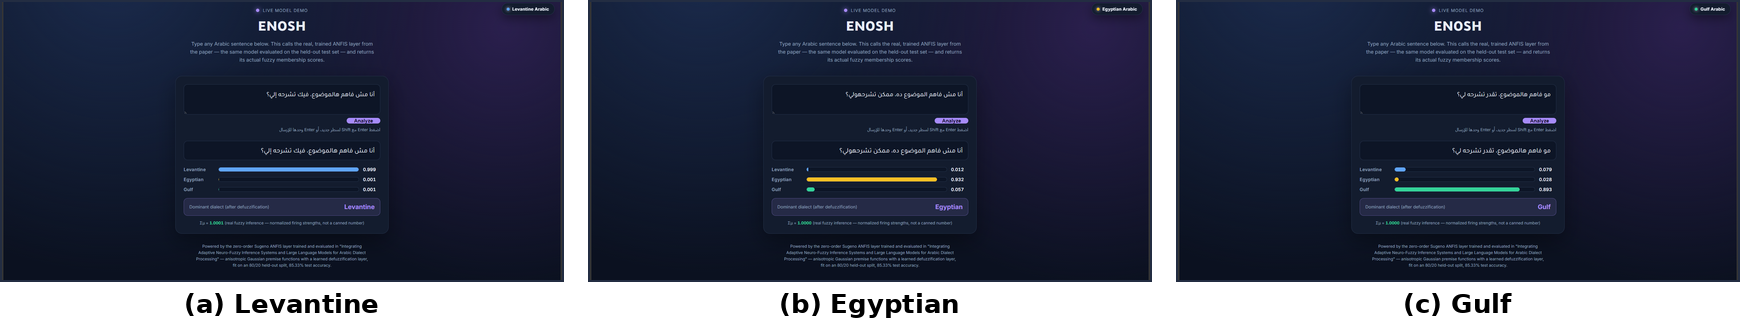
\includegraphics[width=\textwidth]{figure4_enosh_demo.png}
\caption{ENOSH, the live interactive demo backed by the final trained ANFIS model, correctly identifying (a) Levantine, (b) Egyptian, and (c) Gulf Arabic input sentences. The small badge in the top-right corner of each panel surfaces the detected dialect at a glance.}
\label{fig:enosh_demo}
\end{figure*}

Table~\ref{tab:ablation} reports a controlled ablation isolating the two architectural changes introduced in Section~II-A---switching from an isotropic to an anisotropic Gaussian premise, and adding the defuzzification (consequent) layer---evaluated on the identical held-out MARBERT+PCA test split (600 utterances, 200 per dialect).

\begin{table}[t]
\centering
\caption{Ablation: premise type and defuzzification (MARBERT embeddings, identical held-out split)}
\label{tab:ablation}
\begin{tabular}{lc}
\toprule
Configuration & Accuracy \\
\midrule
Isotropic premise, decision from $\mu$ & 0.6500 \\
Isotropic premise + defuzzification & 0.6583 \\
Anisotropic premise, decision from $\mu$ & 0.8583 \\
Anisotropic premise + defuzzification (adopted) & 0.8533 \\
\midrule
$k$-NN ($k$=5) baseline, same embeddings & 0.7900 \\
\bottomrule
\end{tabular}
\end{table}

The anisotropic premise is responsible for essentially the entire improvement: moving from isotropic to anisotropic variance estimation raises accuracy from 65.00\% to 85.83\% on identical embeddings and split, confirming that different PCA dimensions of the MARBERT space carry substantially different dialect-discriminative signal that a single shared per-class variance cannot exploit. The defuzzification layer's own marginal effect is within noise for $n=600$ ($+0.83$ pts isotropic, $-0.50$ pts anisotropic); we report this honestly rather than as an accuracy-improving step, and adopt the anisotropic-plus-defuzzification model (85.33\%) as final since it is architecturally complete and statistically indistinguishable from the simpler anisotropic variant.

Table~\ref{tab:anfis} details the final model's held-out performance, including a macro-F1 of 0.8533, directly answering the request in review for this metric alongside the confusion matrix. The trained ANFIS layer (85.33\%) now exceeds the $k$-NN baseline (79.00\%) by a clear margin---the reverse of the isotropic-premise pattern, where ANFIS and $k$-NN were both mid-40s (Table~\ref{tab:ablation})---indicating the anisotropic form exploits per-dimension class structure more effectively than distance-based neighbor voting, not merely matching it.

To confirm this is not an artifact of the particular 80/20 split, we additionally ran 5-fold stratified cross-validation of the identical model (PCA refit within each fold to avoid leakage). Fold accuracies were 0.8433, 0.8517, 0.8748, 0.8397, and 0.8397: mean accuracy 0.8499 (std 0.0132), mean macro-F1 0.8498 (std 0.0134)---closely matching the single-split result and confirming it generalizes across partitions rather than reflecting one favorable split.

\begin{table}[t]
\centering
\caption{Final ANFIS held-out test performance by dialect (anisotropic premise + defuzzification, MARBERT embeddings)}
\label{tab:anfis}
\begin{tabular}{lccc}
\toprule
Dialect & Precision & Recall & F1-score \\
\midrule
LEV & 0.89 & 0.83 & 0.86 \\
EGY & 0.85 & 0.84 & 0.84 \\
GUL & 0.83 & 0.89 & 0.86 \\
\midrule
\multicolumn{4}{l}{\textbf{Accuracy = 0.8533}, Macro F1-score = 0.8533 (600 test samples)} \\
\multicolumn{4}{l}{$k$-NN ($k$=5) baseline = 0.7900} \\
\bottomrule
\end{tabular}
\end{table}

Table~\ref{tab:confusion} shows the resulting confusion matrix. Unlike the original isotropic-premise result, where GUL was comparatively well separated while LEV and EGY were frequently confused with one another, per-dialect recall is now balanced across all three classes (83--89\%), and the residual confusion is distributed fairly evenly across off-diagonal cells (12--20 misclassifications each) rather than concentrated in one dialect pair, consistent with the anisotropic premise exploiting dialect-specific structure that was not accessible to the earlier isotropic form.

\begin{table}[t]
\centering
\caption{Final ANFIS confusion matrix (rows = true, columns = predicted)}
\label{tab:confusion}
\begin{tabular}{lccc}
\toprule
 & LEV (pred.) & EGY (pred.) & GUL (pred.) \\
\midrule
LEV (true) & 167 & 16 & 17 \\
EGY (true) & 12 & 168 & 20 \\
GUL (true) & 9 & 14 & 177 \\
\bottomrule
\end{tabular}
\end{table}

Qualitative inspection of held-out examples illustrates how $\mu_d$ behaves in the final model: a lexically distinctive utterance received a near-unanimous $\mu_{GUL}=0.963$, while a more ambiguous one received a graded $\mu_{LEV}=0.209$, $\mu_{EGY}=0.161$, $\mu_{GUL}=0.630$---correctly dominant but expressing genuine residual uncertainty, consistent with the fuzzy inter-dialect boundaries of Section~III-B. This is the qualitative signature expected of a layer that has learned genuine dialectal structure rather than memorized surface cues; residual errors elsewhere (Table~\ref{tab:confusion}) show this structure, while now substantially stronger, is not yet perfect.

Fig.~\ref{fig:enosh_demo} shows the trained model running live in ENOSH, our interactive demo built directly on this same anisotropic-premise-plus-defuzzification model: three example sentences, one per dialect, each correctly identified, with the detected dialect surfaced both in the fuzzy-membership panel and in a small always-visible indicator badge.

% ----------------------------------------------------------------------
\section{Limitations and Future Work}
Although this study provides an initial empirical and conceptual foundation for integrating Adaptive Neuro-Fuzzy Inference Systems (ANFIS) with Large Language Models (LLMs) in Arabic dialect processing, several limitations should be acknowledged and addressed in future work.

\subsection{Residual Classification Errors and Scope of the Embedding-Model Swap}
Coupling an anisotropic Gaussian premise with a dialect-specialized embedding model (MARBERT) substantially closed the gap identified in our initial submission, raising held-out accuracy from 46.33\% to 85.33\% with balanced per-dialect recall (83--89\%; Section~III-C). Four limitations remain. First, roughly 15\% of held-out examples are still misclassified (Table~\ref{tab:confusion}); some genuine LEV--EGY--GUL boundary cases persist, consistent with the fuzzy rather than strictly categorical dialect boundaries motivating this work. Second, the defuzzification layer's own contribution to accuracy is within noise for $n=600$ (Table~\ref{tab:ablation}); we report this honestly rather than as an accuracy-improving step, and future work should examine non-linear or jointly-learned premise/consequent parameters \cite{jang1993}. Third, the closed-loop generation pipeline (Fig.~\ref{fig:enosh_demo}) is illustrative rather than systematically evaluated: it depends on a third-party commercial LLM API, and we do not yet report automatic or human quality/fidelity scoring across the full test set, which is left to future work. Fourth, the corpus consists of three hard-labeled parallel dialect variants rather than naturally occurring mixed-dialect utterances with annotated graded membership. As a partial, honest check on this gap, we built a synthetic mixed-dialect probe: splicing the first half of one dialect's utterance with the second half of another's for the same (parallel) held-out test scenario yielded 264 synthetic mixed sentences with a known source pair. The model's average top-membership confidence dropped from 0.868 (pure sentences) to 0.805 (synthetic mixes), and its top-two dialects by membership matched the true spliced pair in 58.0\% of cases---well above the 33\% chance level. This supports the membership degrees carrying genuine, partial signal about mixing, but we do not overclaim: word-splicing is not natural code-switching, no human verified naturalness, and 58\% agreement, while well above chance, is far from perfect. We treat this as suggestive, partial evidence; a genuinely annotated mixed-dialect set, compared against classifier confidence or human judgment, remains the definitive direction for future work. We also note the embedding-model swap was scoped deliberately to the classification sub-task; Sections~III-A--III-B continue to use the original general-purpose embedding model.

\subsection{Further Limitations}
Three additional limitations remain for future work. The analysis covers only three major dialects (LEV, EGY, GUL), omitting Maghrebi, Sudanese, Yemeni, and other varieties, and does not examine MSA--dialect mixing \cite{habash2012}, \cite{altwairesh2018}, \cite{elhaj2021}. The gold corpus, while internally consistent and carefully parallel, is authored by a small number of experts and restricted to short, single-turn exchanges, so it under-represents sociolinguistic diversity, noisy user-generated text, and code-switching; larger, crowd-sourced or naturally occurring corpora are needed to complement it. Finally, the framework is developed only for Arabic; whether it transfers to other dialect-rich languages (e.g., Spanish, Chinese, Hindi, Turkish), and whether complementary cluster-quality metrics or projections such as UMAP would strengthen the embedding-space analysis \cite{vandermaaten2008}, are both left to future work.

% ----------------------------------------------------------------------
\section{Conclusion}
This work addresses a central challenge in Arabic NLP: modeling the rich, overlapping, often fuzzy boundaries between Arabic dialects within dialogue systems. Within this parallel, topic-matched corpus, descriptive PCA/t-SNE analysis suggested GUL forms a comparatively more distinct grouping while LEV and EGY overlap substantially, consistent with prior work \cite{habash2012}, \cite{altwairesh2018}, \cite{elhaj2021}---though we treat this unsupervised analysis as descriptive, not statistical proof of separability (Section~III). The paper's actual quantitative evidence comes from a trained, held-out-evaluated ANFIS classifier: coupling an anisotropic Gaussian premise with a dialect-specialized embedding model (MARBERT) and a learned defuzzification layer achieves 85.33\% three-way accuracy---above a $k$-NN baseline (79.00\%) and with balanced recall (83--89\%)---confirming the fuzzy membership degrees $\mu_d$ carry genuine, learnable dialectal signal rather than remaining a purely conceptual construct, and this result holds under 5-fold cross-validation (0.8499 mean accuracy).

We further instantiated a closed-loop ANFIS--LLM pipeline, converting membership degrees into a dialect-aware steering prompt for an LLM decoder, illustrated on held-out utterances and in ENOSH, our live demo (Fig.~\ref{fig:enosh_demo}); the full implementation is documented in the supplementary material. The observed LEV--EGY overlap, together with a synthetic mixed-dialect probe (Section~IV-A) showing partial but genuine sensitivity to mixing, underscores why graded, fuzzy membership---rather than hard, mutually exclusive labels---is appropriate for real-world Arabic dialogue, where code-switching and gradual transitions between dialects are common. Future work expanding dialectal coverage, diversifying datasets with naturally occurring and mixed-dialect text, and scaling the closed-loop prototype to a systematically evaluated generation study will be important steps toward realizing this approach in practice.

% ----------------------------------------------------------------------
\section*{Acknowledgment}
\subsection*{Disclosure of AI Usage}
While drafting this manuscript, the authors utilized Google Colab and the generative AI tool ChatGPT (OpenAI, San Francisco, USA) to aid in suggesting alternative expressions, condensing text written by the authors (such as the Abstract, Introduction, and Discussion), and ensuring grammatical accuracy and coherence. The authors are solely responsible for all ideas, study design, analyses, and conclusions. Any text generated with AI assistance was thoroughly reviewed, significantly revised, and validated by the authors, who assume full responsibility for the final content.

\subsection*{Funding}
The authors received no financial support for the research, authorship, and/or publication of this article.

\subsection*{Declaration of Conflicting Interests}
The authors declared no potential conflicts of interest with respect to the research, authorship, and/or publication of this article.

\subsection*{Supplemental Material}
Supplemental material for this article is available online at \url{https://github.com/enosh-science}.

% ----------------------------------------------------------------------
\begin{thebibliography}{00}
\bibitem{abdulmageed2021} M. Abdul-Mageed, A. Elmadany, and E. M. B. Nagoudi, ``ARBERT \& MARBERT: Deep bidirectional transformers for Arabic,'' in \textit{Proc. 59th Annual Meeting of the Association for Computational Linguistics and the 11th International Joint Conference on Natural Language Processing (ACL-IJCNLP 2021)}, 2021, pp. 7088--7105.
\bibitem{altwairesh2018} N. Al-Twairesh, H. Al-Khalifa, and M. Al-Razgan, ``A survey on Arabic dialect identification,'' \textit{International Journal of Computer Science Issues}, vol. 15, no. 1, pp. 1--10, 2018.
\bibitem{elhaj2021} M. El-Haj, P. Rayson, and H. Al-Khalifa, ``Arabic dialect identification,'' in \textit{The Oxford Handbook of Arabic Linguistics}, E. Benmamoun and R. Bassiouney, Eds. Oxford, U.K.: Oxford Univ. Press, 2021, pp. 576--595.
\bibitem{habash2012} N. Habash, M. Diab, and O. Rambow, ``Conventional approaches to Arabic natural language processing,'' \textit{Computational Linguistics}, vol. 38, no. 3, pp. 531--579, 2012.
\bibitem{jang1993} J.-S. R. Jang, ``ANFIS: Adaptive-network-based fuzzy inference system,'' \textit{IEEE Trans. Systems, Man, and Cybernetics}, vol. 23, no. 3, pp. 665--685, 1993.
\bibitem{jolliffe2002} I. T. Jolliffe, \textit{Principal Component Analysis}, 2nd ed. New York, NY, USA: Springer, 2002.
\bibitem{reimers2019} N. Reimers and I. Gurevych, ``Sentence-BERT: Sentence embeddings using Siamese BERT-networks,'' in \textit{Proc. 2019 Conf. Empirical Methods in Natural Language Processing (EMNLP)}, 2019, pp. 3982--3992.
\bibitem{vandermaaten2008} L. van der Maaten and G. Hinton, ``Visualizing data using t-SNE,'' \textit{Journal of Machine Learning Research}, vol. 9, pp. 2579--2605, 2008.
\end{thebibliography}

\end{document}
